% !TeX root = RJwrapper.tex
\title{APCI: An R and Stata Package for Visualizing and Analyzing Age-Period-Cohort Data}
\author{by Jiahui Xu, Liying Luo}

\maketitle

\abstract{
Social scientists have frequently attempted to assess the relative contribution of age, period, and cohort variables to the overall trend in an outcome. We develop an R package \CRANpkg{APCI} (and Stata command \code{apci}) to implement the age-period-cohort-interaction (APC-I) model for estimating and testing age, period, and cohort patterns in various types of outcomes for pooled cross-sectional data and multi-cohort panel data. Package \CRANpkg{APCI} also provides a set of functions for visualizing the data and modeling results. We demonstrate the usage of package \CRANpkg{APCI} with empirical data from the Current Population Survey. We show that package \CRANpkg{APCI} provides useful visualization and analytical tools for understanding age, period, and cohort trends in various types of outcomes.
}

\section{Introduction} \label{introduction}

Researchers across disciplines have long been interested in distinguishing the relative contribution of three time-related variables — namely, age (i.e., how old a person is at the time of data collection), time periods (e.g., the Great Recession 2007-2009 and the COVID-19 pandemic beginning in December 2019), and cohort membership (e.g., the baby boom cohort born in 1945-1964 and the Millennials born in 1981-1996) — to the overall trends in various outcomes (e.g., labor force participation, attitudes, and cognitive functioning) \citep{alwin_generations_2003, clogg_cohort_1982,pescosolido2021trends}.  Decomposing the overall trends into age, period, and cohort variations provides insight into the ways in which biological and social factors affect these outcomes \citep{hobcraft_age_1982, heckman_using_1985, fosse_analyzing_2019}. 

To quantify the relative contribution of age, period, and cohort, \citet{luo_age-period-cohort-interaction_2020} have recently developed a model called the age-period-cohort-interaction (APC-I) model. The APC-I is qualitatively different from other age-period-cohort (APC) models in that it characterizes cohort effects as a structure of the age-by-period interaction terms to acknowledge the interdependence of age, period, and cohort effects, whereas prior methods attempt to recover the independent and additive effects of the three variables. The APC-I model has been used to understand the unique contribution of cohort membership in various outcomes including crime involvement, substance use, and cultural taste \citep{lu_cohort_2020, verdery_visualizing_2020, ma_what_2020}. However, the authors of the APC-I model focused on the conceptual motivation of the method and offered relatively few technical details for implementing the method.  Estimating and testing cohort effects in the APC-I model may be be challenging for interested readers.  

We developed an R package \CRANpkg{APCI} \citep{apci} and a Stata command \code{apci} for implementing the APC-I model in empirical research using pooled cross-sectional data (e.g., the General Social Survey and the Current Population Survey) and importantly, extend the APC-I method for analyzing multi-cohort longitudinal or panel data (e.g., data from the Health and Retirement Study (\hyperlink{https://hrs.isr.umich.edu/about}{HRS}) and the National Longitudinal Study of Youth (\hyperlink{https://www.bls.gov/nls/}{NLSY})). The purpose of this paper is three folded. First, we describe the R functions in the \CRANpkg{APCI} package and Stata command to estimate and test age, period, and cohort effects in the APC-I model.  The core function can be used for analyzing pooled cross-sectional data and multi-cohort longitudinal data.  Second, we introduce a set of visualization tools to help researchers motivate an APC analysis and interpret age, period, and cohort effects from the APC-I model.  Third, we clarify several important issues about characterizing cohort effects as a set of age-by-period interaction terms. We pay particular attention to the implications of coding schemes and how to interpret the between-cohort average deviations and within-cohort life-course variations. 

This paper is organized as follows. Following a description of traditional APC models and the identification problem, we introduce the APC-I model and the estimation and testing procedures.  We explain how and why the age-by-period interaction terms can be used to characterize cohort effects with particular attention to the implications of coding schemes for estimating and testing interactions.  Next, we describe the visualization tools and functions in the R package \CRANpkg{APCI}.  We then demonstrate how to use the package with the empirical example of men's and women's labor force participation from 1990 to 2018 in the United States using data from the Current Population Survey \citep[\hyperlink{https://www.census.gov/programs-surveys/cps/data.html}{CPS,}][]{cps_citation}.

\section{Methodology: the APC-I model} \label{methodology}
\subsection{The APC identification problem} \label{identification}

To formally estimate and infer the independent age, period, and cohort effects, \citet{mason_methodological_1973} specified an analysis of variance (ANOVA) model that they labeled the age-period-cohort (APC) accounting model:

\begin{equation} \label{eq:1}
g\left(E\left(Y_{i j}\right)\right)=\mu+\alpha_{i}+\beta_{j}+\gamma_{k}
\end{equation}
for age groups $i=1, 2,\ldots, A$, periods $j=1, 2,\ldots, P$, and cohorts $k=1, 2,\ldots, (A+P-1)$, where $\sum_{i=1}^{A} \alpha_{i}=\sum_{j=1}^{P}\beta_{j}=\sum_{k=1}^{A+P-1} \gamma_{k}=0$. $E\left(Y_{i j}\right)$denotes the expected value of the outcome $Y$ for the $i$th age group in the $j$th time period; $g$ is the ``link function''; $\alpha_i$ denotes the mean difference from the global mean $\mu$ associated with the $i$th age category; $\beta_j$ denotes the mean difference from $\mu$ associated with the $j$th period; $\gamma_k$ denotes the mean difference from $\mu$ associated with membership in the $k$th cohort.  

Unfortunately, the APC accounting model (\ref{eq:1}) is not identified even when a coding scheme (e.g., dummy coding where one group is set as the reference group or effect coding where the sum of the coefficients for each effect is set to 0) is applied. This is because age, period, and cohort are exactly linearly related \citep[see][for detailed discussions]{fienberg_identification_1979,fosse_analyzing_2019,luo_sensitivity_2016}. As a result, the design matrix of model (\ref{eq:1}) has rank one less than full, so an infinite number of solutions (i.e., estimates) for the parameters fit the data equally well.  That is, the data cannot distinguish different estimation results, so an additional constraint — in addition to the usual reference group or sum-to-zero constraint — must be imposed in order to choose one set of estimates.  Moreover, interpreting the results is difficult because the standard interpretation of regression coefficients — that is, the conditional effect of one variable after accounting for other covariates — cannot apply due to the lack of variation in the third variable (e.g., cohort) after considering the other two (e.g., age and period).


The theoretical root of the identification problem in traditional APC models is the problematic assumption that age, period, and cohort effects operate independently of each other. It implies that the identification challenge is inherent in any APC model that attempts to separate independent and additive effects of age, period, and cohort and thus cannot be solved by changing the model setup \citep[e.g., using random effects for period and cohort as in \citealp{yang_mixed_2006}; see][for a critique]{luo_constraints_2020} or by variable manipulation \citep[e.g., using unequal interval widths for age, period, and cohort groups as in \citealp{robertson_age_1986,sarma_canadian_2012}; see][for a detailed discussion]{luo_sensitivity_2016}.  The identification problem is well recognized, and its consequences have been discussed extensively \citep{fienberg_specification_1985, fosse_analyzing_2019, kupper_age-period-cohort_1983,kupper_statistical_1985, luo_sensitivity_2016, luo_constraints_2020, te_grotenhuis_intrinsic_2016, obrienEstimableIntraageIntraperiod2020, morgan2021rolling,luo2013paradigm}. In essence, internal information derived from the data cannot help because the problem is circular: researchers do the analysis to learn precisely the kind of information needed to justify any such constraint.




\subsection{The APC-I model} \label{model}

\citet{luo_age-period-cohort-interaction_2020} proposed a new APC model called the age-period-cohort-interaction (APC-I) model. The APC-I model is qualitatively different from all estimators developed under the traditional framework in that it explicitly specifies cohort effects as a structure of the age-by-period interactions. A life-course dynamics hypothesis that concerns about whether and how cohort effects may change as cohorts age thus corresponds to a specific structure of the age-by-period interactions. This specification is motivated by the theoretical account that ``The minimal basis for expecting interdependence between inter-cohort differentiation and social change is that change has variant import for persons of unlike age'' \citep{ryder_cohort_1965}. That is, a basic notion on which cohort analysis rests is that ``transformations of the social world modify people of different ages in different ways.'' \citep{ryder_cohort_1965}

The APC-I model is fully identified in the sense that it does not require additional constraints other than a regular coding scheme. It is also flexible enough to test various hypotheses about life-course changes within cohorts as cohort members age.  We first describe the model specification and estimation and testing techniques.  The next section demonstrates the procedure using empirical examples. 

The general form of the APC-I model can be written as:
\begin{equation} \label{eq:2}
g\left(E\left(Y_{i j}\right)\right)=\mu+\alpha_{i}+\beta_{j}+\alpha \beta_{i j(k)}
\end{equation}
where $g$, $Y_{ij}$, $\mu$, $\alpha_{i}$ and $\beta_{j}$ are defined as in model (\ref{eq:1}) and $\alpha \beta_{i j(k)}$ denotes the interaction of the $i$th age group and $j$th period group, corresponding to the effect of the $k$th cohort. Note that except for the oldest and youngest cohorts, the effect of one cohort includes multiple age-by-period interaction terms $\alpha \beta_{i j(k)}$ that lie on the same diagonal in a table with ages in rows and periods in columns.  

Model (\ref{eq:2}) differs from model (\ref{eq:1}) in the way that cohort effects are modeled. In model (\ref{eq:2}), cohort effects are considered as a specific form of the age-by-period interaction. In statistics, the interaction between two variables describes the differential effects of one variable depending on the level of the other \citep{scheffe_analysis_1999}.  In APC research, this means that if part of the overall pattern of interest can be attributed to cohort differences, significant age-by-period interactions should be present.  When cohort membership is not associated with the outcome — that is, when the effects of historical or social shifts (period effects) are uniform across age groups — then age-by-period interactions should not be present.   

\citet{luo_age-period-cohort-interaction_2020} described a procedure for investigating age and period main effects and inter-cohort deviations and intra-cohort dynamics.  They recommended beginning with a deviance test about whether the effects of time periods vary among age groups, which is called ``a global F test''. A non-significant global F statistic indicates that there are few age-by-period interaction effects and thus little cohort variation.  If the model suggests significant age-by-period interaction effects, one may proceed to examine inter- and intra-cohort differences\footnote{The local deviation test is unavailable in the current version (1.0.5) of the R package that we develop.}.  Inter-cohort average deviations are quantified based on the arithmetic mean of the age-by-period interaction terms contained in each cohort and a t test can be used to examine the average of that cohort-specific deviation.  To investigate intra-cohort dynamics over the life course \citep[e.g., the cumulative (dis)advantage hypothesis in][]{dannefer_aging_1987, ferraro_what_2018,chauvelTestingPersistenceCohort2016,obrienEstimableIntraageIntraperiod2020}, one may use a t-test of the linear orthogonal polynomial contrast in each cohort's age-by-period interaction effects.  This intra-cohort life-course dynamics test is helpful for investigating whether the average (dis)advantages of the members of that cohort accumulate, remain stable, or diminish as they age.

The APC-I model has three advantages.  First, it is identified in that it does not require additional constraints other than the usual coding scheme. That is, it avoids the identification problem of the APC accounting model based on the theoretical account of cohort effects and allows inclusion of other important predictors such as education, sex, and employment status.  Second, the interpretation of the coefficient estimates of the APC-I model is meaningful and straightforward.  This is because the APC-I model recognizes the dependence of age, period, and cohort so the dilemma that analysts face using traditional APC models does not apply. Third, the APC-I model permits investigating life-course dynamics as a cohort ages, whereas extant methods usually assume that cohort effects do not change.

It is important to note that the APC-I model is never intended to "solve" the identification problem in traditional APC accounting models because it is a false problem to begin with. Given the near monopoly of the accounting model, it may be challenging not to see the APC-I method through the lens of the traditional APC accounting framework. For example, because the APC-I model quantifies cohort effects as a structure of the age-by-period interactions, some readers may take it to mean that the APC-I model cannot estimate "linear cohort main effects". However, the APC-I method, by design, does not intend to estimate any kind of "linear cohort main effects" precisely because the traditional model's assumption that there is a linear cohort effect that is additive or independent of age and period effects lacks theoretical grounding and is thus arbitrary and questionable. Please see \citet{luo_age-period-cohort-interaction_2020} for a more thorough discussion about the theoretical motivation of the APC-I model. 

Because the APC-I mode is relatively new, below we make additional remarks about interaction effects and coding schemes to help readers better understand and use the model.  

\subsection{Interaction effects} \label{interaction}

In some cases, interaction terms may be difficult to interpret besides suggesting that the effect of one variable may depend on the values of the other.  However, as explained by \citet{luo_age-period-cohort-interaction_2020}, the age-by-period interaction terms correspond to the conceptual definition of cohort effects and thus can be modeled and interpreted in a meaningful way.  Specifically, cohort effects are expected when the influence of social events and changes differ by age groups.  This conceptualization of cohort effects implies that the age-by-period interactions, which represent the differential effects of time periods depending on age, can be used to measure cohort effects. 

Technically, because of the linear dependency among age, period, and cohort, the effects of the third variable can be expressed as the interaction between the other two variables.  The APC-I model considers age and period as main effects and cohort their interactions, which may give the impression that it privileges age and period effects and ``discriminates'' against cohort effects.  The theoretical motivation for this choice is that it is often desirable to estimate a general age pattern that individuals follow as they get older.  Period main effects are used to represent the kind of impacts of social environment that everyone in the society is exposed to.  The decision to quantify cohort effects as a specific form of age-by-period interaction is informed by the demographic literature on how cohort effects are conceptualized in relation to age and period effects.  Empirically, as the analysis of women's labor force participation in section \hyperref[example]{Examples} will illustrate, the size of the cohort effects, characterized as the age-by-period interactions, is not necessarily smaller—in fact may be larger—than some of the main effects.  

\subsection{Coding scheme and contrast} \label{contrasts}

For the unidentified APC accounting model, some estimation methods including the intrinsic estimator yield effect estimates that are dependent on the choice of coding schemes in that estimates under different coding schemes are not equivalent \citep[see][for a more detailed discussion]{luo_sensitivity_2016, te_grotenhuis_intrinsic_2016}. The APC-I model does not have a rank deficiency problem in the sense that it does not require more constraints than a usual ANOVA model with main effects and their interactions.  For any identified model including the APC-I model, the estimates are equivalent; that is, the estimated cell means are the same for all coding schemes.  

Although this equivalence holds for both main effects and interaction estimates in the APC-I model, it is less obvious for interaction terms because the interpretation of the specific parameter estimates do change with coding schemes.  To illustrate, consider an example of applying the APC-I model to health data with three age categories and three periods, shown in \hyperref[table:1]{table 1} below.  Under dummy coding—for example, the youngest age group 20-24 and the beginning survey period of 2000 are set to zero or omitted as the referent—the interaction for ages 25-29 and period 2005 in cell Y represents the difference in a health outcome between periods 2000 and 2005 for age 25-29 or equivalently, health difference between ages 25-29 and 20-24 for the period 2005.  That is, interactions under dummy coding represents a directional difference from a particular reference group.  

\begin{center}
$$
\begin{array}{|c|c|c|c|c|}
\hline & & \multicolumn{3}{|c|} {\text { Period }}  \\
\hline & & 2000 & 2005 & 2010 \\
\hline \text { Age } & 20-24 & & & \\
\cline { 2 - 5 } & 25-29 & & \mathrm{Y} & \\
\cline { 2 - 5 } & 30-34 & & & \\
\hline
\end{array}
$$
\captionof{table}{Hypothetical data with three age categories and three periods illustrating a shift in meaning and interpretation of interaction terms under different coding schemes. The interaction terms under different types of coding in cell Y necessarily have different numerical values because of different reference groups. For example, the interaction term in cell Y under dummy coding represents a directional difference from a particular reference group (e.g., age 20-24 in year 2000). Under effect coding, the same interaction term in cell Y represents the deviation in the outcome from the age main effect plus period main effect for the group of individuals who were age 25-29 and surveyed in period 2005. Such different numeric values do not arise from an identification problem but rather from a shift in what these quantities represent. }
\label{table:1}
\end{center}

By contrast, under effect coding (i.e., sum-to-zero coding), the same interaction term in cell $Y$ represents the deviation in the health outcome from the age main effect plus period main effect for the group of individuals who were age 25-29 and surveyed in period 2005. 

The estimated interaction terms under these two types of coding in cell $Y$ thus necessarily have different numerical values. However, this difference does not arise from an identification problem but rather from a shift in what these quantities represent.  That is, the two interaction terms can be transformed to be equivalent so that the means in $Y$ after considering age and period main effects are the same under the two coding schemes.  

We recommend using effect or sum-to-zero coding for estimating the APC-I model for the following reasons: when characterizing cohort effects as a set of age-by-period interactions, we are less concerned about any direction of the interactions; that is, we are not particularly interested in the difference between two cohorts at a particular age or time period.  Rather, we focus on particular structures of these interactions that may represent theoretically interesting patterns during a cohort's life span.  Effect coding is helpful because they all have the same referent group — the next lower level in the hierarchy of main effects and interactions. That is, we choose effect coding for the purpose of easy interpretation.  This is also consistent with the recommendation of coding schemes in the presence of interactions \citep{aiken_multiple_1991, jaccard_interaction_2003}.  

\section{The R package APCI} \label{pacakge}

\subsection{Package installation} \label{install}

The R package \CRANpkg{APCI} \footnote{The R package \CRANpkg{APCI} works well in R version above 3.6.0., but updating to the latest version of R is highly recommended.} can be installed and loaded using the following R code\footnote{If users have never installed packages in R or RStudio, use the following R code instead: \code{install.packages("APCI", repos = "http://cran.us.r-project.org")}.                                           }:
\begin{example}
# install R package APCI
> install.packages("APCI")
# load R package APCI to the current working environment 
> library(APCI)
\end{example}

The main routines to implement the APC-I model using package \CRANpkg{APCI} are \code{apci.plot.raw}, \code{apci}, \code{apci.plot} (or \code{apci.plot.hexagram}, \code{apci.plot.heatmap}). A summary of these functions and input arguments used in the routines are described below.

\subsection{Functions in R package APCI} \label{functions}

The R package \CRANpkg{APCI} contains the following functions for estimating the APC-I model and visualizing the data and the model results:

\begin{itemize}
\item {\code{apci}}: to estimate the age, period, and cohort effects using the APC-I model.
\item{\code{temp\_model}}: an internal function that estimates a generalized linear model.
\item {\code{tests}}: to conduct the global F test.
\item{\code{maineffect}}: an internal function to extract age and period main effects. 
\item{\code{cohortdeviation}}: an internal function to extract between-cohort average deviations and within-cohort life-course dynamics.
\item{\code{ageperiod\_group}}: to return a cohort index based on how age and period are grouped. 
\item {\code{apci.plot.raw}}: to visualize the mean values of the outcome across age and period groups, respectively. 
\item {\code{apci.plot.hexagram}}: to visualize the estimated cohort effects in a hexagram style.
\item {\code{apci.plot.heatmap}}: to visualize the estimated cohort effects in a heatmap style.
\item {\code{apci.plot}}: to visualize the estimated age, period, and cohorts in conventional figures.
\end{itemize}

A summary of input arguments required in these functions will be given one by one \footnote{Summaries for internal functions are not listed. Please see \href{https://cran.r-project.org/web/packages/APCI/APCI.pdf}{APCI reference manual} for details about internal functions.} in the next section. Package \CRANpkg{APCI} also contains three empirical datasets \textit{women9017}, \textit{cpsmen}, \textit{cpswomen}, and one simulated dataset \textit{simulation}. Dataset \textit{women9017} was used and described in \citet{luo_age-period-cohort-interaction_2020}. Applications of the APC-I model to the other two empirical datasets are given in section \hyperref[example]{Examples}.

\subsubsection{Function apci} \label{fun:apci}

Function {\code{apci}} is the core function in the R package \CRANpkg{APCI}. It fits an APC-I model with or without covariates and returns a list of results including coefficients and standard error estimates for age main effects, period main effects, inter-cohort average deviations, and intra-cohort life-course trends, and covariate coefficients if any. Both pooled cross-sectional data and multi-cohort longitudinal/panel data are supported. Specifically, function {\code{apci}} is used as 

\begin{example}
	apci(data, outcome, age, period, cohort, weight, covariate, family, 
		dev.test=TRUE, print, gee, id, corstr,...)
\end{example}

and takes the following arguments:

\begin{itemize}
\item {\code{data}}: a data frame containing an outcome variable, age group indicators, period group indicators, and covariates to be used in the model. If a variable is not found in data, there will be an error message reminding users to check the input data again. Supported data structures include pooled cross-sectional data and multi-cohort longitudinal/panel data. 

\item {\code{outcome}}: an object of class character containing the name of the outcome variable. The outcome variable can be a continuous, categorical, or count variable. 

\item {\code{age}}: an object of class character indicating the age group index taking on the number of distinct values in the data (e.g., six age groups: 20-24, 25-29, 30-34, 35-39, 40-44, and 45-49). The vector should be a factor (or ``category'', or ``enumerated type'').

\item {\code{period}}: an object of class character indicating the time period index in the data.

\item {\code{cohort}}: an optional object of class character indicating cohort membership index in the data. The cohort index can be generated from the age group index and time period index in the data because of the exact linear relationship among these three time-related indices.

\item {\code{weight}}: an optional vector of sample weights to be used in the model fitting process. If {\code{non-NULL}}, user-supplied weights will be used in the first step to estimate the model. Observations with negative weights will be dropped in modeling.

\item {\code{covariates}}: an optional vector of characters containing the names of user-specified covariate(s) to be used in the model. If the variables are not found in data, there will be an error message reminding the users to check the data again.

\item {\code{dev.test}}: logical, specifying if the global F test (step 1) should be implemented before fitting the APC-I model. If {\code{TRUE}}, {\code{apci}} will first run the global F test and report the test results; otherwise, {\code{apci}} will skip this step and return {\code{NULL}}. The default setting is {\code{TRUE}}. However, users should be aware that the algorithm will not automatically stop even if there is no significant age-by-period interactions based on the global F test.\footnote{The following error may appear: ``Error in solve.default(V): `a' is 0-diml''. To address this error, users may bypass the F test by setting the argument \code{dev.test} to {\code{FALSE}}.}

\item {\code{family}}: a character string specifying the link function to be used in the model. The value can be ``binomial'', ``multinomial'', or ``gaussian''. See R function \code{glm} for more details about link functions.

\item {\code{print}}: logical, specifying if the intermediate results should be displayed in the console when fitting the model. The default setting is {\code{TRUE}} to display the results of each procedure.

\item {\code{gee}}: logical, indicating if the data is cross-sectional data or longitudinal/panel data. If {\code{TRUE}}, the generalized estimating equation will be used to correct the standard error estimates. The default is {\code{FALSE}}, indicating that the data are cross-sectional.

\item {\code{id}}: a character vector specifying the cluster index in longitudinal data. It is required when {\code{gee}} is {\code{TRUE}}. The length of the vector should be the same as the number of observations.

\item {\code{corstr}}: a character string specifying a possible correlation structure in the error terms when {\code{gee}} is {\code{TRUE}}. The following are allowed: {\code{independence}}, {\code{fixed}}, {\code{stat\_M\_dep}}, {\code{non\_stat\_M\_dep}}, {\code{exchangeable}}, {\code{AR-M}} and {\code{unstructured}}. The default value is {\code{exchangeable}}. 

 \item{\code{unequal\_interval}}: logical, indicating if age and period groups are of the same interval width. The default is set as \code{TRUE}.
 
 \item{\code{age\_range, period\_range}}:
numeric vectors indicating the actual age or period range (e.g., 10 to 59 years old or from 2000 to 2019).
  
  \item{\code{age\_interval, period\_interval, age\_group, period\_group}}:{
numeric values or character vectors indicating how age and period are
grouped. \code{age\_interval} and \code{period\_interval} 
indicate the width of age and period intervals, respectively. \code{age\_group} and \code{period\_group} are character vectors listing possible age and period groups. There are two ways to define age and period groups with unequal intervals: 1) defining \code{age\_interval} and \code{period\_interval}, or 2) defining \code{age\_group} and \code{period\_group}. Users must define age and period groups using one of the two options when \code{unequal\_interval} is \code{TRUE}.
  }
\item {\code{...}}: further optional arguments to be passed to the model. 

\end{itemize}

As mentioned in section \hyperref[contrasts]{Coding scheme and contrast}, we use  effect coding to estimate the APC-I model. The {\code{age}} and {\code{period}} arguments in function {\code{apci}} accept categorical variables. Different from the common approach of dummy coding or simple coding, where an effect is defined as the difference of each group from the reference group, function {\code{apci}} uses effect coding (i.e., the sum-to-zero coding, deviation coding, or the ANOVA coding) as the default coding. Under this coding scheme, the effect of the omitted category equals the negative sum of the effects of all other categories. Computation wise, the effect coefficient of the omitted category is redundant because of the coding scheme. However, for the purpose of quantifying cohort effects as deviations from the main effects of age and period, it is useful to compute estimates for all age-by-period cross-classifications and their standard errors. For data with \textit{A} age groups and \textit{P} periods, therefore, function {\code{apci}} returns $A$ and $P$ number of main effect estimates and $A*P$ number of interaction estimates along with their standard error estimates. For the main effects of age or period, the estimate can be interpreted as the deviation associated with each age or period group from the global mean.  The age-by-period interactions represent the deviation from the expectation determined by the corresponding age and period main effects.  

Also note that when age and period groups have unequal interval widths in an age-period classification table, the age-by-period interactions contained in a cohort no longer lie on the same diagonals. Because cohort effects are conceptualized and estimated as a structure of the age-by-period interactions in the APC-I model, it is technically possible to use the argument {\code{unequal\_interval}} in package \CRANpkg{APCI} to extract interaction coefficient estimates that lie on different diagonals. However, unequal age and period group intervals may complicate the issue of cohort overlapping noted by \citet{kupper_statistical_1985}.  For this reason, we do not recommend using unequal interval widths for age and period groups if possible. 

After fitting the APC-I model, function {\code{apci}} will store the following components as a list for further usage:
\begin{itemize}
\item {\code{model}}: a summary of the fitted generalized linear regression model.\footnote{\CRANpkg{APCI} supports all types of generalized linear regression models.} It displays the standard regression output including coefficient and standard errors estimates.

\item {\code{dev\_global}}: the global F test results. It examines if the interaction terms are significant in a generalized linear regression model that contains age and period main effects and their interactions.

\item {\code{intercept}}: the overall intercept ($\mu$ in equation \ref{eq:2}).

\item {\code{age\_effect}}: a vector containing the estimated effect for each age group.

\item {\code{period\_effect}}: a vector containing the estimated effect for each time period.

\item {\code{cohort\_average}}: a vector containing the inter-cohort average deviations for comparing differences between cohorts.

\item {\code{cohort\_slope}}: a vector containing intra-cohort life-course trends.

\end{itemize}


\subsubsection{Function tests} \label{fun:tests}
As mentioned earlier, the first step of implementing the APC-I model is to conduct a global F test of the age-by-period interactions. This step is a routine in function {\code{apci}}, but the procedure does not stop even if there is no statistically significant deviation from the age main effect and period main effect. Therefore, we recommend separately conducting the global F test. In R package {\CRANpkg{APCI}}, the function {\code{tests}} can be used for this purpose. It can be used as follows:
\begin{example}
	tests(model, A, P, C, ...)
\end{example}

and takes the following arguments:

\begin{itemize}
\item {\code{model}}: a generalized linear regression model generated from the internal function {\code{temp\_model}}. \footnote{{\code{temp\_model} is an internal function in R package \CRANpkg{APCI}} that accepts the same input arguments as those in function {\code{apci}}. Detailed syntax of this function can be found in \href{https://cran.r-project.org/web/packages/APCI/APCI.pdf}{APCI reference manual}.}

\item {\code{A, P, C}}: numbers of age groups, period groups, or cohort groups. If age and period groups are of different widths, the values of will be automatically generated by the function.

\end{itemize}

Function {\code{tests}} will return a standard F test result including the value of the F test statistic and the associated p-value.


\subsubsection{Functions for visualization} \label{fun:vis}

In package {\CRANpkg{APCI}}, we provide four functions to facilitate visualizing the data and model results, namely {\code{apci.plot.raw}}, {\code{apci.heatmap}}, {\code{apci.plot.hexagram}}, and {\code{apci.plot}}, in different stages of a research project. They take similar input arguments. A summary of these arguments is given below. 


Function {\code{apci.plot.raw}} is designed to plot the outcome variable aggregated by age or period groups. This function may be used in the stage of data exploration. Functions {\code{apci.heatmap}} and {\code{apci.plot.hexagram}} are designed to plot the age-by-period interactions from the APC-I model. Both functions generate heatmaps, where one axis represents age groups, and the other period groups. The cells in a diagonal represent one cohort. The difference between the two functions is the layout of the heatmap; one is a rectangular graph and the other a hexagram. Function {\code{apci.plot}} can be used to visualize both raw data and model results. It divides the canvas into four ($2 \times 2$) panels.  Three of the four panels can be used to visualize the three effect estimates in the APC-I model and the left panel to add notes. For data exploration, users can visualize the mean values of the outcome variable across age, period, and cohort groups on the same canvas. Users can the same functions to visualize the estimated age, period, and cohort effects from the modeling results.

The visualization functions in package {\CRANpkg{APCI}} include:
\begin{example}
	apci.plot.raw(data, outcome_var, age, period, ...)

	apci.plot.heatmap(model, age, period, color_map = NULL, color_scale = NULL, 
		quantile = NULL, ...)

	apci.plot.hexagram(model, age, period, first_age, first_period, interval, 
		color_scale = NULL, color_map = NULL, quantile = NULL, …)

	apci.plot(model, age, period, outcome_var, type = "model", quantile = NULL, 
		...)

\end{example}

and takes the following arguments:

\begin{itemize}
\item {\code{model}}: a list recording the results from function {\code{apci}}.

\item {\code{outcome\_var}}: an object of class character indicating the name of the outcome variable used in the model. The outcome variable can be a continuous, binary, categorical, or count variable.

\item {\code{age}}: a vector indicating the age group. The vector should be converted to a factor (or the terms of ``category'' and ``enumerated type'').

\item {\code{period}}: a vector indicating the time period. The vector should be converted to a factor (or ``category'',  ``enumerated type'').

\item {\code{color\_map}}: a vector representing a color palette to be used in the figure. The default setting is greys if {\code{color\_map}} is {\code{NULL}}. Alternatives, for example, can be c(``blue'', ``yellow''), ``blues'', etc. 

\item {\code{cohort\_scale}}: a vector containing two values to indicate the minimum and maximum values, respectively, of the estimated cohort effects to be displayed. If {\code{NULL}}, the function will use the range from the estimation results.

\item {\code{quantile}}: a number valued between 0 and 1, representing the desirable percentiles to be used in visualizing the data or model. If {\code{NULL}}, the original scale of the outcome variable will be used. 

\end{itemize}

\section{Examples: Application of the R package APCI to empirical data} \label{example}

We now illustrate how to use package {\CRANpkg{APCI}}'s visualization and analytical functions.  We describe and analyze two empirical datasets to demonstrate how this package may be used to analyze pooled cross-sectional data. We later briefly describe how to fit an APC-I model for multi-cohort longitudinal data. 






\subsection{Cross-sectional data of labor force participation in the United States} \label{example1}

Temporal trends in men's and women’s labor force participation (LFP) in United States have gathered much scholarly attention \citep[see e.g.][]{connellyEffectChildCare1992, farkas1977cohort, hollisterUnmaskingConflictingTrends2014, macunovichRelativeCohortSize2012, treasEffectWomenLabor1987, wilkieDeclineMenLabor1991a}. For example, whereas men's LFP steadily declined in the past decades \citep{wilkieDeclineMenLabor1991a}, women’s LFP continued to rise until the 1990s and the 2000s. Female LFP has since then reached a plateau and even begun to decline. Researchers have debated about the causes of this leveling off or decline. Some studies attributed the observed trends to period-specific factors such as labor demand \citep{ercegLaborForceParticipation2014}, the economic shocks of the Great Recession \citep{ bousheyAreWomenOpting, hoffman2009changing}, social welfare and disability insurance \citep{duggan200911}, and gender role attitudes \citep{fortinGenderRoleAttitudes2015}.

However, the temporal trends in LFP are unlikely due to a pure period process. For example, because individuals may begin to leave the labor force in age 50, a decline in LFP should be expected if the proportion of the population age 50 or older has increased. That is, the recent trends may reflect a change in the age composition of the US population \citep{aaronsonLaborForceParticipation2014}. The cohort succession may also contribute to the trend, a process in which older cohorts with higher or lower LFP rates begin to decease and younger cohorts with lower or higher LFP enter the labor force \citet{lee_plateau_2014}. At the same time, critical social and demographic changes in education level, fertility, and attitudes about women working outside the home may be more of cohort-specific than period-specific processes because these forces only affect individuals of certain ages \citep{balleerLabourForceParticipation2014, farreIntergenerationalTransmissionGender2013, fernandezCulturalChangeLearning2013, goldin_quiet_2006}.

Given that the observed trends in LFP are likely a mix of age, period, and/or cohort patterns, an APC analysis that decomposes the temporal trends into age-, period-, and cohort-related variations is thus helpful for revealing the demographic, social, and economic changes that have underlined the temporal trends in American's labor force participation. In this following section, we demonstrate how to use the functions in \CRANpkg{APCI} to undertake an APC analysis of men's and women’s LFP using a cross-sectional dataset.    

The Current Population Survey \citep[\hyperlink{https://www.census.gov/programs-surveys/cps/data.html}{CPS,}][]{cps_citation} is the primary source of labor force statistics in the United States \citep{cps_citation}. Beginning in the 1960s, the CPS has been collecting data on key demographic, economic, and education topics. We subset the 1990-2019 CPS data by gender, resulting in two datasets, namely \textit{cpsmen} and \textit{cpswomen}, to show how to conduct an APC-I analysis of men's and women's LFP in the United States using package \CRANpkg{APCI}. 

Datasets \textit{cpsmen} and \textit{cpswomen} contain a subset of men and women age 20-64 who participated in the 1990 to 2019 CPS. The following code is used to load the data into the working environment:

\begin{example}
> data(cpsmen)
> data(cpswomen)
\end{example}

The first five rows of the datasets of \textit{cpsmen} and \textit{cpswomen} are: 

\begin{example}
> head(cpsmen, n = 5)
  asecwt year age labforce educc
 2854.84    3   5        0     1
 1576.54    4   4        1     2
 2340.55    2   6        1     3
  158.44    3   5        0     0
  347.09    6   6        1     3

> head(cpswomen, n = 5)
  asecwt year age labforce educc
 2415.67    2   3        1     1
  663.89    2   5        1     3
 1653.01    6   4        1     2
 1613.31    6   4        0     2
  177.23    4   3        1     2
\end{example}
where {\code{labforce}} indicates the respondent's labor force participation status (1=in the labor force, 0=not in the labor force). {\code{asecwt}} is the person-level weight that the CPS recommends to be used in individual-level data analyses. {\code{year}} indicates the survey year when respondent was interviewed, grouped into 6 period groups (1=1990-94, 2=1995-99, …, 6=2015-19). {\code{age}} indicates the respondent’s age categories (1=20-24, 2=25-29, …, 9=60-64). {\code{educc}} is a three-level categorical education measure (1=less than high school, 2=high school graduate, 3=college degree or above).  

For data exploratory purpose, function {\code{apci.plot.raw}} visualizes the outcome variable in the following way:
\begin{example}
> apci.plot.raw(data, outcome_var, age, period)
\end{example}

% \begin{center}
%   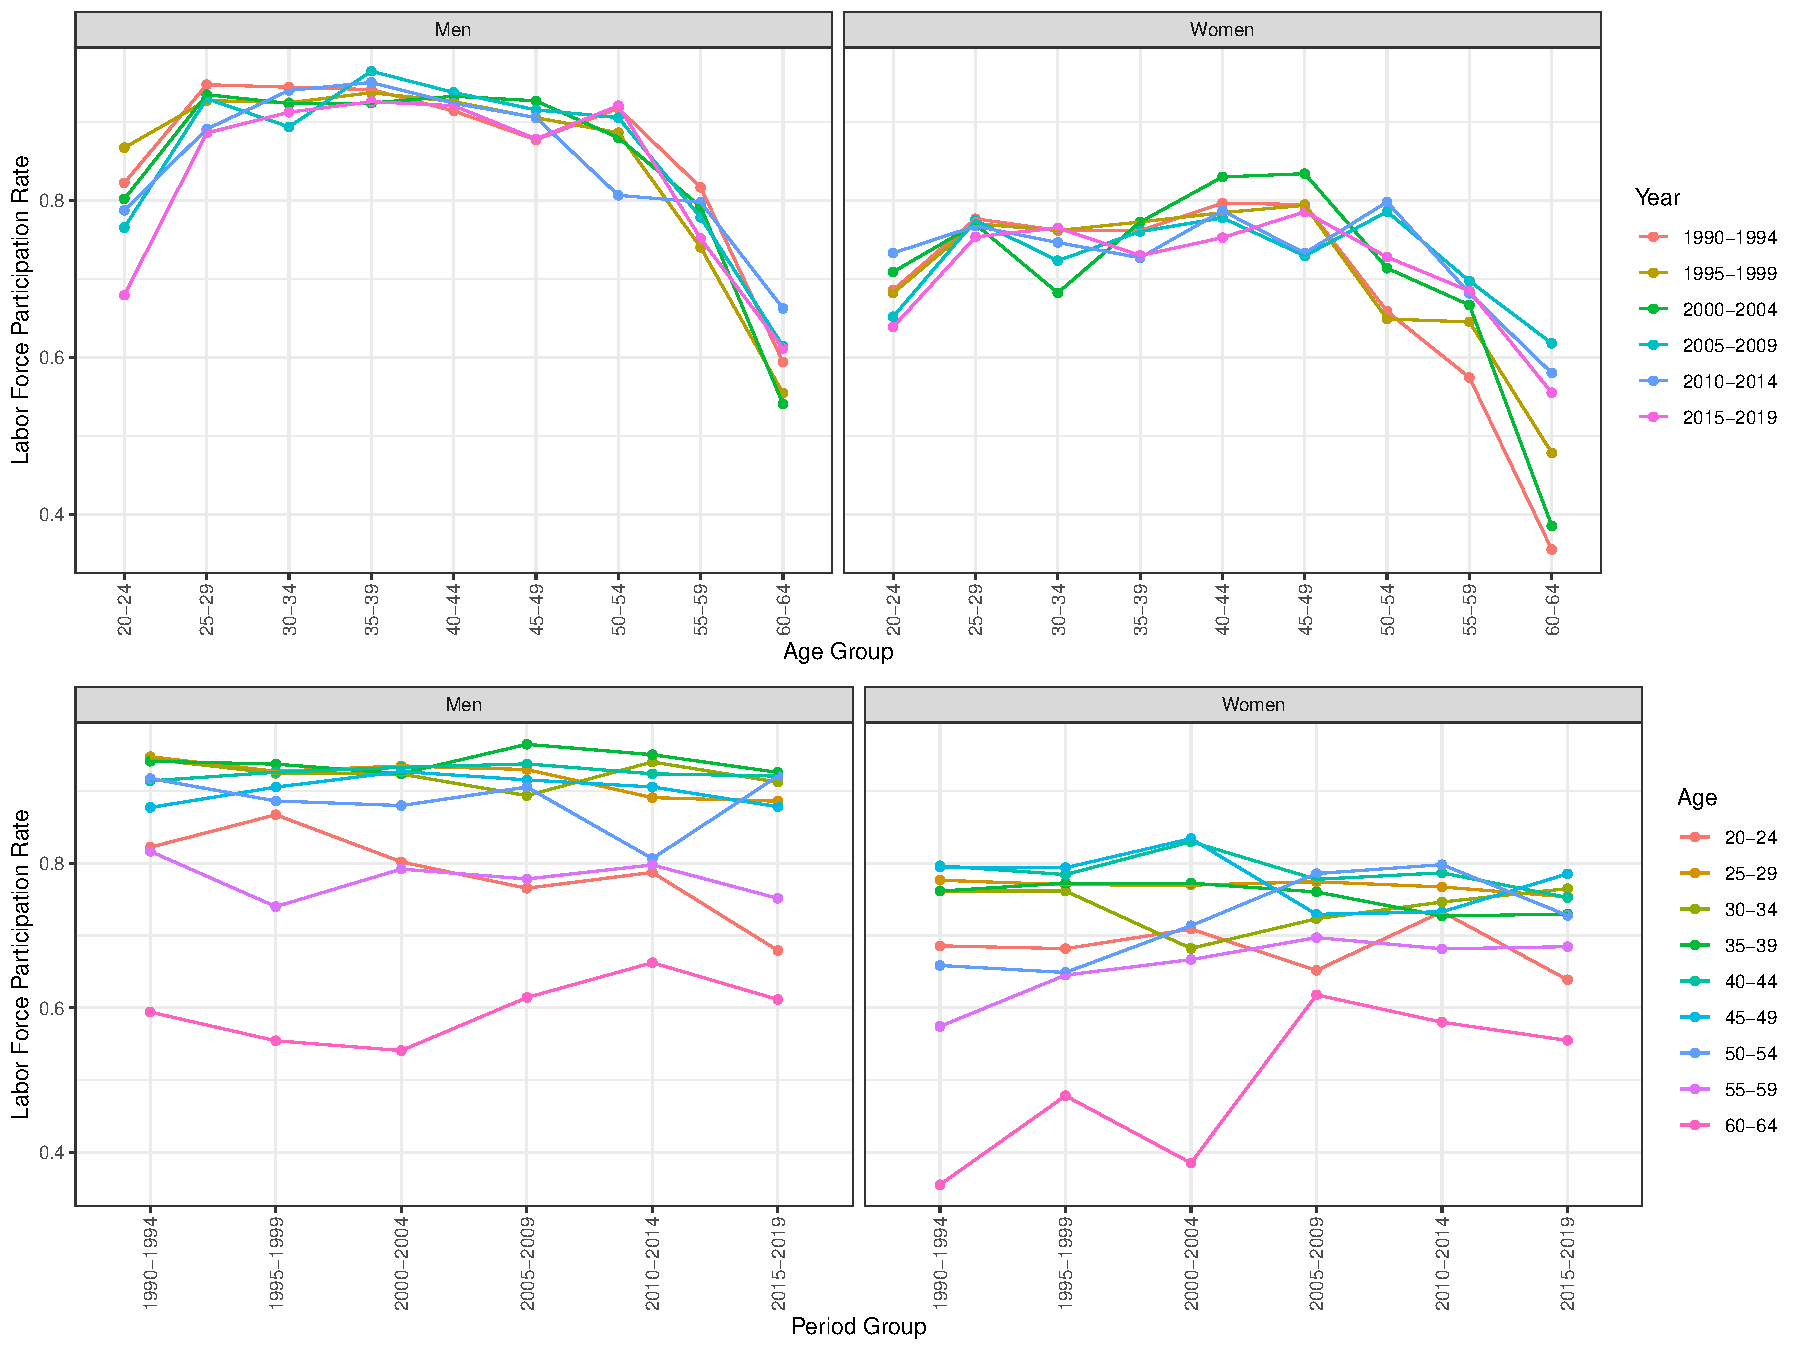
\includegraphics[width=1\linewidth]{figure1.pdf}
% \captionof{figure}{Period-specific age trajectories and age-specific period trends in labor force participation rates for men and women in the United States, the CPS 1990-2019. Age trajectories are similar across time periods for both men and women (top panel). Period trends differ by age groups, especially among women (bottom panel).}\label{figure:1}
% \end{center}

\begin{figure}[htbp]
  \centering
  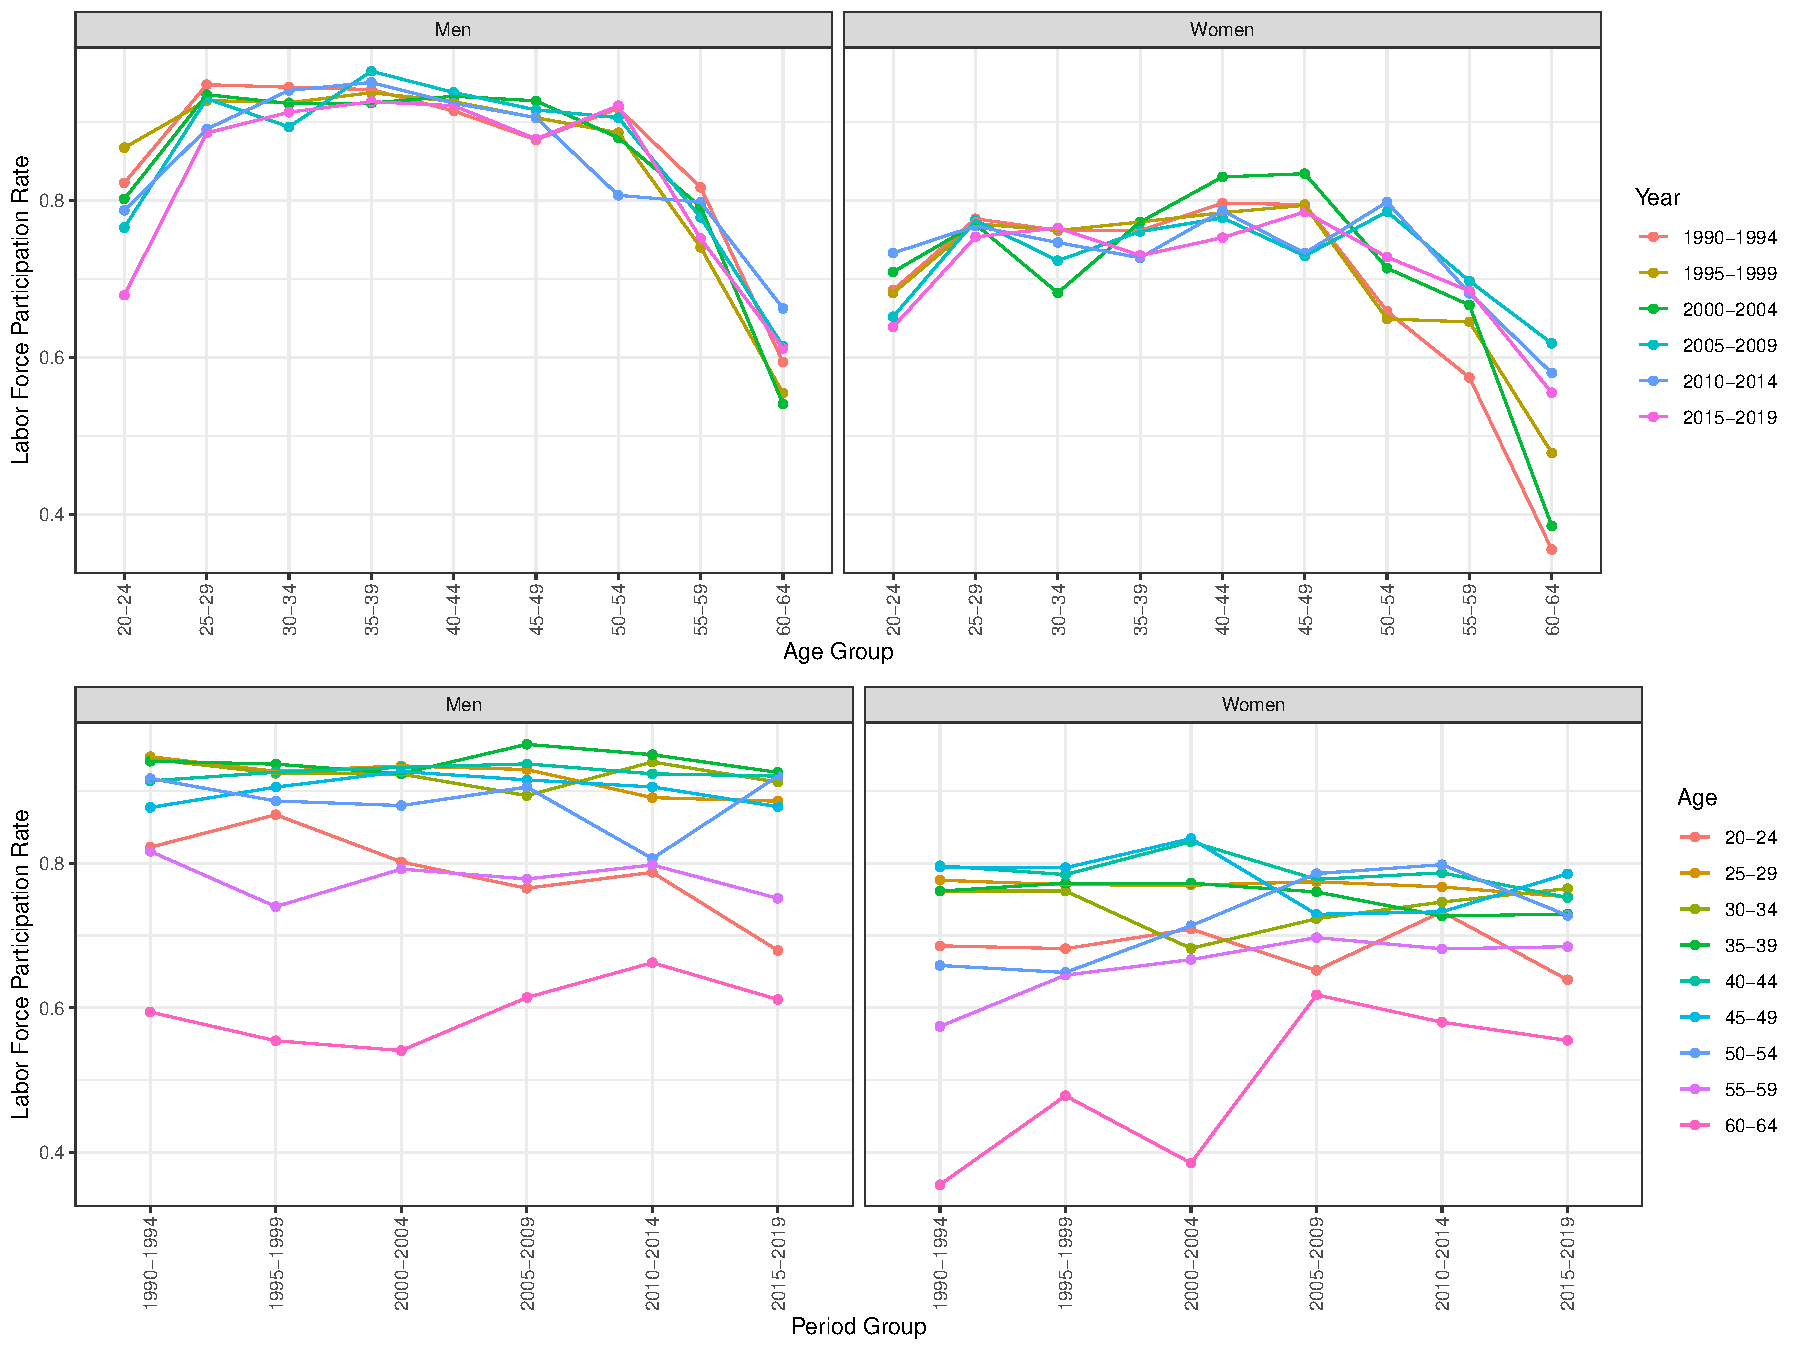
\includegraphics[width=1\linewidth]{figure1.pdf}
  \caption{Period-specific age trajectories and age-specific period trends in labor force participation rates for men and women in the United States, the Current Population Survey 1990-2019. Age trajectories are similar across time periods for both men and women (top panel). Period trends differ by age groups, especially among women (bottom panel).}
  \label{figure:1}
\end{figure}

\hyperref[figure:1]{Figure 1} shows LFP rates by age groups (top panel) and period groups (bottom panel), respectively, for male (left panel) and female CPS respondents (right panel) age 20 to 64 from 1990 to 2019. Figure 1's top panel suggests similar age patterns in LFP across time periods. The bottom panel shows distinct period trends depending on age groups. For example, the LFP rates among women in the 55-59 and 60-64 age groups seem to have gone up whereas other age groups show a relatively flat trend. Such distinct period patterns in LFP by age groups suggest potential cohort variations in women's labor force participation. For men's LFP, however, the visualization results suggest that a simpler model with age and period main effects may suffice for summarizing their LFP patterns. 

Function {\code{apci}} can be used to fit an APC-I model for pooled cross-sectional data or multi-cohort longitudinal/panel data. In the simplest form of an APC-I model without covariates for pooled cross-sectional data, function {\code{apci}} is called as follows:

\begin{example}
> no_cov <- APCI::apci(outcome = "labforce", 
+                      age = "age", 
+                      period = "year", 
+                      weight = "asecwt",
+                      data = cpswomen, 
+                      dev.test = FALSE, 
+                      family = "binomial")
\end{example}

It is often desirable to add covariates in the model, which can be done by calling the {\code{covariate}} argument.  For example, suppose one would like to add education levels (``educc'') as a covariate in the model, function {\code{apci}} can be used as:

\begin{example}
> with_cov <- APCI::apci(outcome = "labforce",
+                        age = "age",
+                        period = "year",
+                        covariate = c("educc"),
+                        weight = "asecwt",
+                        data = cpswomen, 
+                        print=F,
+                        dev.test=FALSE, 
+                        family = "binomial")
\end{example}

Below is a summary of the results from an APC-I model that includes education levels as a covariate:

\begin{example}
> summary(with_cov)
               Length Class      Mode     
model          33     svyglm     list     
dev_global      0     -none-     NULL     
intercept       4     -none-     character
age_effect     45     -none-     character
period_effect  30     -none-     character
cohort_average  6     data.frame list     
cohort_slope    6     data.frame list     
int_matrix      5     data.frame list     
cohort_index   54     -none-     numeric  
data            7     data.frame list   
\end{example}

The returned value is a list of objects. \code{model} contains the results from a logistic regression model with age and period main effects and the unstructured interactions. \code{dev\_global} displays the global F test result. A significant F statistic suggests that there may exist cohort effects. \code{intercept} is the overall intercept ($\mu$ in Equation \ref{eq:2}). \code{age\_effect} gives estimated age main effect. \code{period\_effect} is the estimated period main effect.  \code{cohort\_average} gives inter-cohort average deviations from age and period main effects.  \code{cohort\_slope} gives intra-cohort life-course linear slopes, which can be used for testing intra-cohort life-course dynamics. \code{int\_matrix} displays a matrix that contains the estimated coefficients for age-by-period interactions.  Note that there are A*P interactions in \code{int\_matrix} because effect coding is used to compute the A+P-1 interaction estimates based on the (A-1)*(P-1) freely varying interaction parameters. Such interaction estimates are used to generate heatmaps similar to Figure 2. \code{data} stores the data fed into \code{apci} function. Users may call an object to obtain detailed results. For example, by calling {\code{with\_cov\$cohort\_average}} and {\code{with\_cov\$cohort\_slope}}, users can obtain estimated inter-cohort average deviations and intra-cohort life-course slopes.

The output below shows education-adjusted inter-cohort average deviations in women's LFP from analyzing the \textit{cpswomen} data using function {\code{apci}}.

\begin{example}
> with_cov$cohort_average
   c_avg_group c_avg_est c_avg_se c_avg_t c_avg_p c_avg_sig
1            1    -0.329    0.193  -1.709   0.088          
2            2    -0.155    0.142  -1.091   0.275          
3            3    -0.162    0.114  -1.422   0.155          
4            4     0.047    0.097   0.481   0.631          
5            5     0.096    0.085   1.139   0.255          
6            6     0.174    0.076   2.288   0.022       *  
7            7     0.034    0.074   0.457   0.648          
8            8    -0.036    0.074  -0.493   0.622          
9            9     0.003    0.073   0.047   0.963          
10          10    -0.072    0.081  -0.894   0.371          
11          11     0.030    0.085   0.353   0.724          
12          12    -0.029    0.102  -0.288   0.774          
13          13    -0.080    0.131  -0.609   0.543          
14          14    -0.103    0.170  -0.608   0.543          
\end{example}
where \code{c\_avg\_group} indicates cohort membership (e.g., cohort 1=the 1930 birth cohort, cohort 2=the 1935 birth  cohort,...,cohort 14=the 1995 birth cohort), \code{c\_avg\_est} is inter-cohort average deviation, \code{c\_avg\_se} is the standard error estimate for the average deviation, \code{c\_avg\_t} is the t test statistic for the average deviation, and \code{c\_avg\_p} and \code{c\_avg\_sig} are the p values and alpha levels (*: p < .05, **: p < .01, and ***: p < .001), respectively. 

The results from \code{with\_cov\$cohort\_average} imply that on average, the LFP rates among cohort 6's--the 1955 birth cohort -- significantly differ from the expected rates based on age and period main effects. Specifically, the 1955 cohort shows a .19 (exp(.174)-1, p < .05) higher participation rate than the expectation based on the age and period main effects. 

The output below shows education-adjusted intra-cohort life-course dynamics in women's LFP from analyzing the \textit{cpswomen} data using function {\code{apci}}.

\begin{example}
> with_cov$cohort_slope
   c_slp_group c_slp_est c_slp_se c_slp_t c_slp_p c_slp_sig
1            1        NA       NA      NA      NA      <NA>
2            2     0.165    0.195   0.849   0.396          
3            3    -0.215    0.187  -1.148   0.251          
4            4     0.163    0.189   0.866   0.386          
5            5     0.093    0.184   0.508   0.611          
6            6     0.007    0.169   0.039   0.969          
7            7     0.047    0.172   0.277   0.782          
8            8    -0.096    0.181  -0.530   0.596          
9            9    -0.187    0.173  -1.076   0.282          
10          10    -0.106    0.176  -0.602   0.547          
11          11    -0.279    0.159  -1.750   0.080          
12          12     0.353    0.160   2.207   0.027       *  
13          13    -0.047    0.180  -0.262   0.793          
14          14        NA       NA      NA      NA      <NA>
\end{example}
where \code{c\_slp\_group} indicates cohort membership (e.g., cohort 1=the 1930 birth cohort, cohort 2=the 1935 birth cohort,..., cohort 14=the 1995 birth cohort), \code{c\_slp\_est} is intra-cohort life-course slopes, \code{c\_slp\_se} is the standard error estimate for the life-course slope, \code{c\_slp\_t} is the t test statistic for the life-course slope, and \code{c\_slp\_p} and \code{c\_slp\_sig} are the p values and alpha levels (*: p < .05, **: p < .01, and ***: p < .001), respectively. \code{NA}s are generated for the youngest and oldest cohort because there is only one age-by-period combination observed for the two cohorts and thus intra-cohort life-course dynamics cannot be accessed. 

For example, for cohort 12 (the 1985 birth cohort), the estimated intra-cohort slope is 0.353 (p < .05), meaning that this cohort's LFP is lower than expected when they were young but higher than expected in older ages. Interestingly, for cohort 12 (the 1985 birth cohort), their average cohort deviation is not statistically significant. Such an insignificant inter-cohort average deviation and a significantly negative intra-cohort slope indicate a compensation life-course pattern; that is, this cohort's lower-than-expected LFP in younger ages seems to be compensated by their higher LFP when they were older. 

The intra-cohort life-course dynamics are based on the age-by-period interactions as follows:

\begin{example}
# the first six rows of the life-course dynamics
> with_cov$int_matrix 
  iaesti  iase   iap iasig cohortindex
1  0.166 0.169 0.327                 9
2 -0.048 0.207 0.818                 8
3  0.068 0.164 0.678                 7
4  0.095 0.172 0.581                 6
5  0.205 0.191 0.283                 5
6  0.227 0.193 0.239                 4
# [there are 48 rows compressed]
\end{example}
where ``iaesti'' is the age-by-period interaction estimates, ``iase'' is the standard error estimate for the interaction term, ``iap'' and ``iasig'' are the p value and alpha level (*: p < .05, **: p < .01, and ***: p < .001),respectively, and ``cohortindex'' indicates cohort membership. 

The following code can be used to organize the intra-cohort life-course estimates in a matrix form:

\begin{example}
> matrix(with_cov$int_matrix, A, P)[A:1,] 
# A is the number of age groups and P is the number of period groups.

       period #1 period #2 period #3 period #4 period #5 period #6
age #9 -0.329    -0.038    -0.416*    0.334     0.267     0.182   
age #8 -0.272     0.043     0.017     0.125     0.001     0.086   
age #7 -0.112    -0.392*   -0.070     0.257     0.278     0.040   
age #6  0.227    -0.046     0.443*   -0.333*   -0.258    -0.033   
age #5  0.205     0.066     0.061    -0.150    -0.074    -0.107   
age #4  0.095     0.044     0.139     0.065    -0.109    -0.234   
age #3  0.068     0.059    -0.359*   -0.147     0.096     0.283   
age #2 -0.048     0.256    -0.006     0.067    -0.156    -0.113   
age #1  0.166     0.009     0.191    -0.216    -0.046    -0.103 
\end{example}

Based on the R package {\CRANpkg{ggplot2}} \citep{ggplot2}, heatmaps can be generated to visualize inter- and intra-cohort patterns and motivate a subsequent formal APC analysis. For example, for dataset \textit{whitemen}, both inter-cohort average deviations and intra-cohort life-course dynamics may be visualized in a heatmap as follows:

\begin{example}
> apci.plot.heatmap(model = with_cov, age = "age",period = 'year',
                  color_map = c('blue','yellow'))
\end{example}

% \begin{center}
%   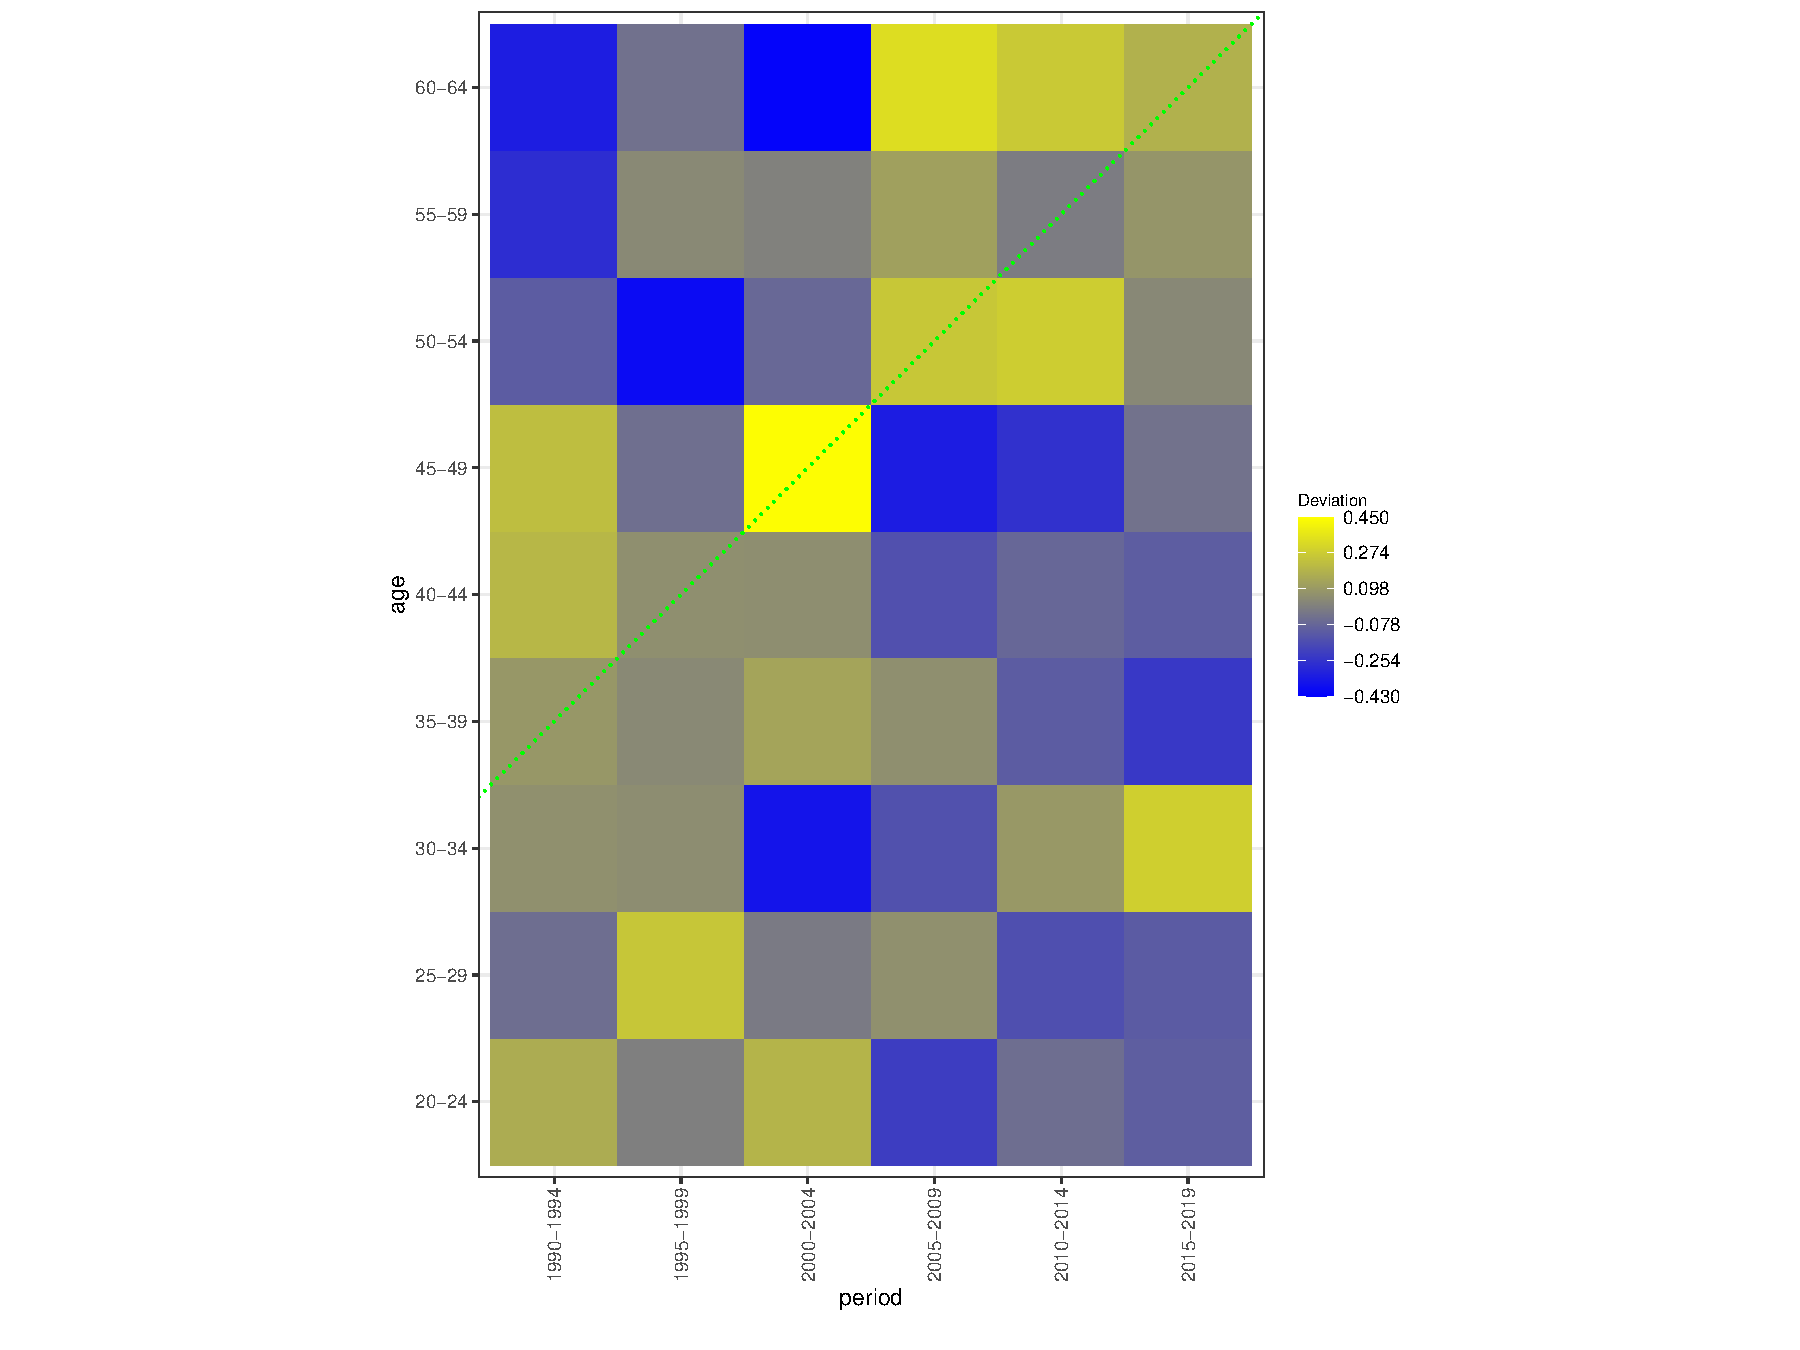
\includegraphics[width=1\linewidth]{figure2.pdf}
% \captionof{figure}{Cohort deviations heatmap showing higher-than-expected labor force participation rates that persists over their life course for the 1955 birth cohort.  Each square represents an age-by-period interaction. Yellow squares indicate lower participation rates than the expectation determined by the age and period main effects. Blue squares indicate higher-than-expected rates. Each diagonal that runs from the lower left to the upper right represents one birth cohort. The dotted line indicates a significant average inter-cohort deviation but an insignificant intra-cohort slope in their labor force participation rates for the 1955 cohort.}\label{figure:2}
% \end{center}

\begin{figure}[htbp]
  \centering
  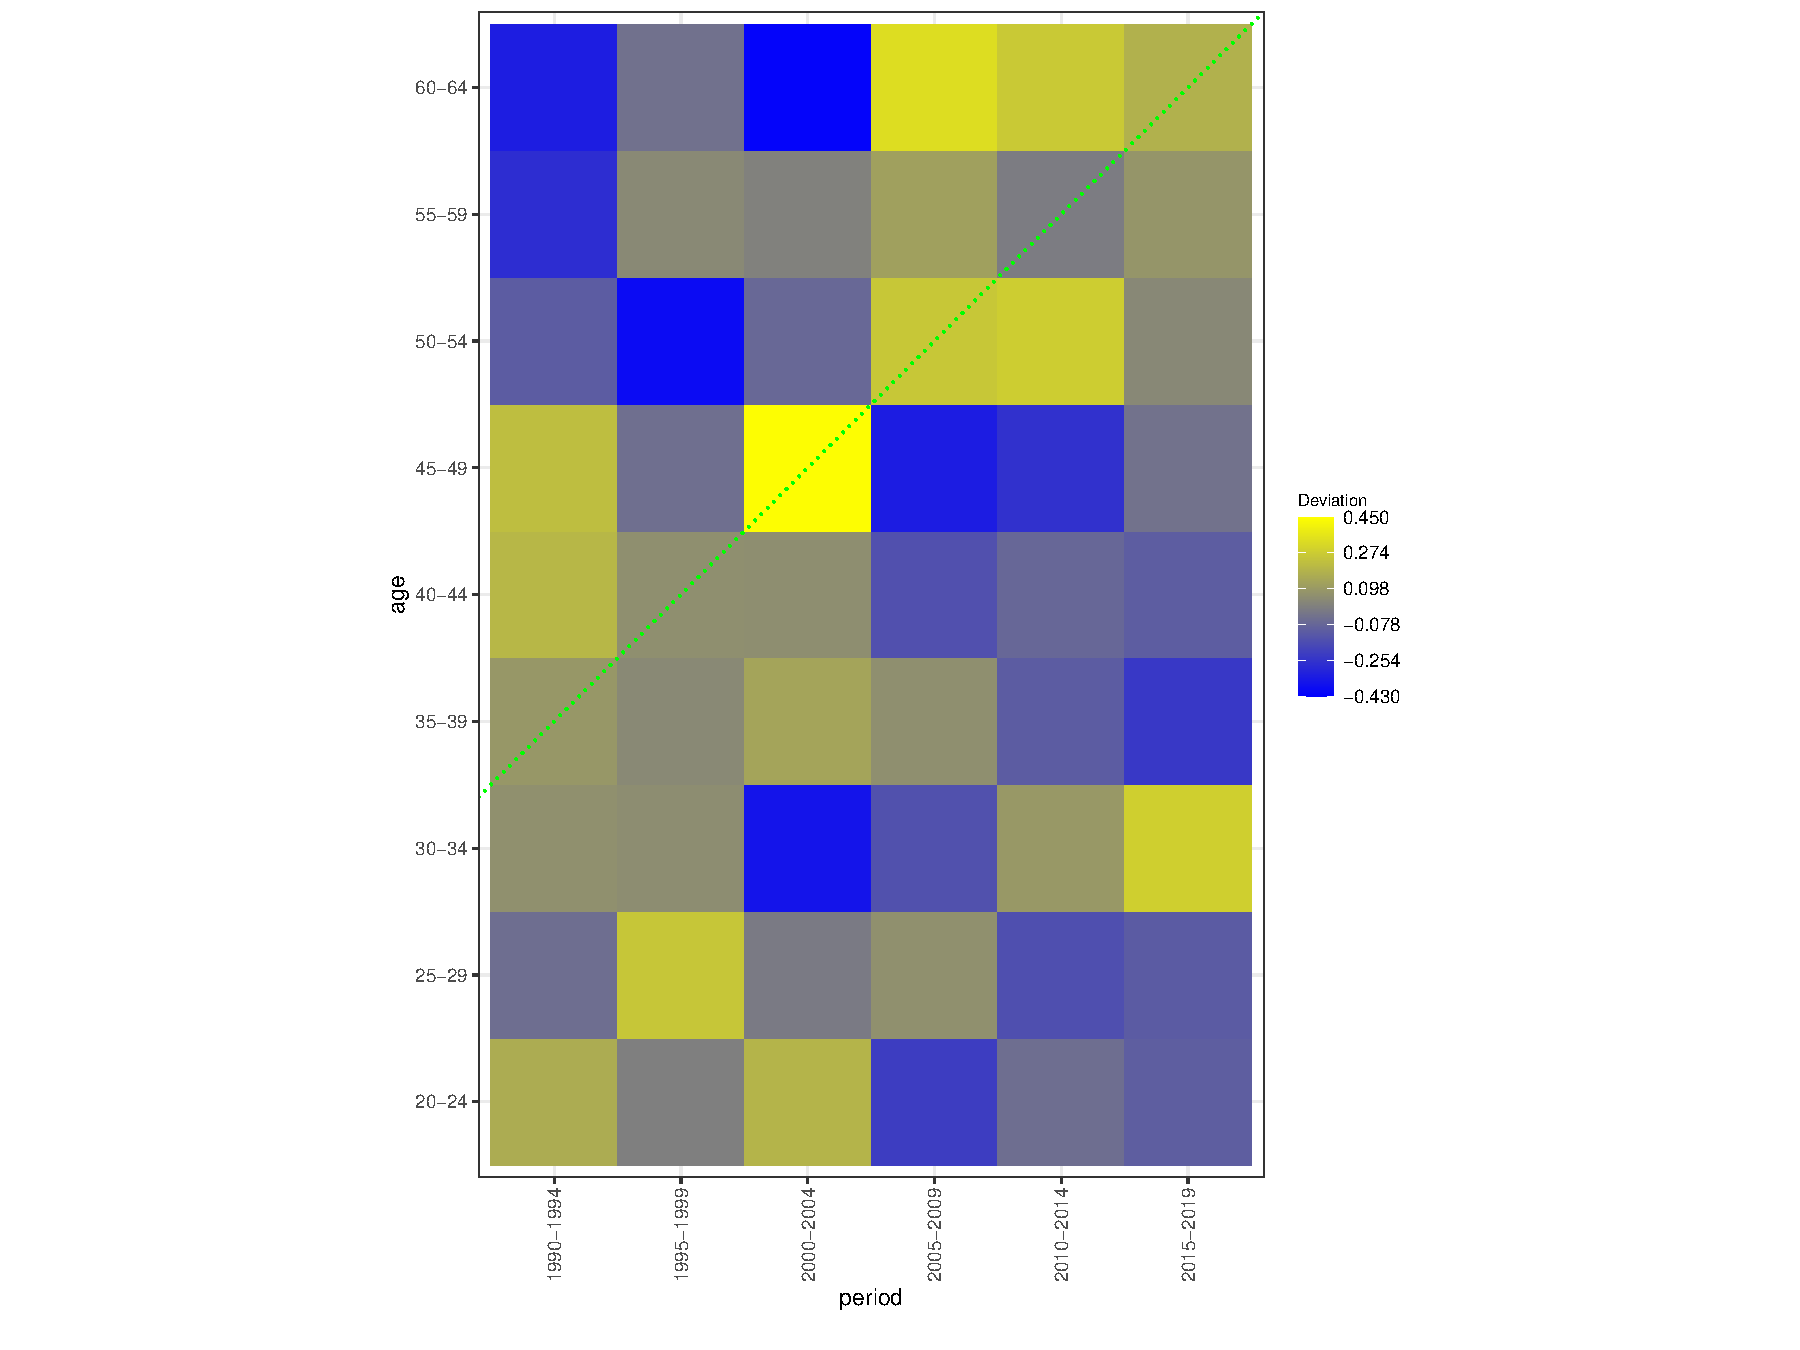
\includegraphics[width=1.2\linewidth]{figure2.pdf}
  \caption{Cohort deviation heatmap showing higher-than-expected labor force participation rates that persist over their life course for the 1955 birth cohort.  Each square represents an age-by-period interaction. Yellow squares indicate lower participation rates than the expectation determined by the age and period main effects. Blue squares indicate higher-than-expected rates. Each diagonal that runs from the lower left to the upper right represents one birth cohort. The dotted line indicates a significant average inter-cohort deviation but an insignificant intra-cohort slope in their labor force participation rates for the 1955 cohort.}
  \label{figure:2}
\end{figure}

\hyperref[figure:2]{Figure 2} is a heatmap of the estimated age-by-period interactions, with rows defined by age groups and columns by time periods. Each square represents an age-by-period interaction. Yellow squares indicate lower participation rates than the expectation determined by the age and period main effects. Blue squares indicate higher-than-expected rates. Each diagonal that runs from the lower left to the upper right represents one birth cohort. The dotted line in Figure 2 indicates a significant inter-cohort average deviation but an insignificant intra-cohort slope in their LFP for the 1955 cohort. Cohorts that on average significantly deviate from the expected rates based on age and period main effects are indicated by solid, dashed, or dotted lines. Solid lines indicate significantly (p<.05) positive intra-cohort life-course slopes, dashed lines significantly negative intra-cohort slopes, and dotted lines significant average inter-cohort deviations but insignificant intra-cohort slopes. Users have the options to customize the elements of these figures to suit their research or teaching purposes.

Figure 2 indicates that although some cohorts had LFP rates that differ from the expected rates based on age and period main effects, only the 1955 birth cohort (marked by a dotted line) had, on average, higher-than-expected LFP rates (inter-cohort average deviation = .174, p < .05), and this higher LFP seems to persist over their life course (intra-cohort slope = .007, p = .969). This visualization results are consistent with the results from \code{with\_cov\$cohort\_average} and \code{with\_cov\$cohort\_slope}.

Users can also use bar plots to visualize inter-cohort average deviations. Function {\code{apci.bar}} can be used as:
\begin{example}
> apci.bar(model = with_cov, age = "age",period = "year", 
            cohort_label = seq(1930,1995,5))
\end{example}

\begin{figure}[htbp]
  \centering
  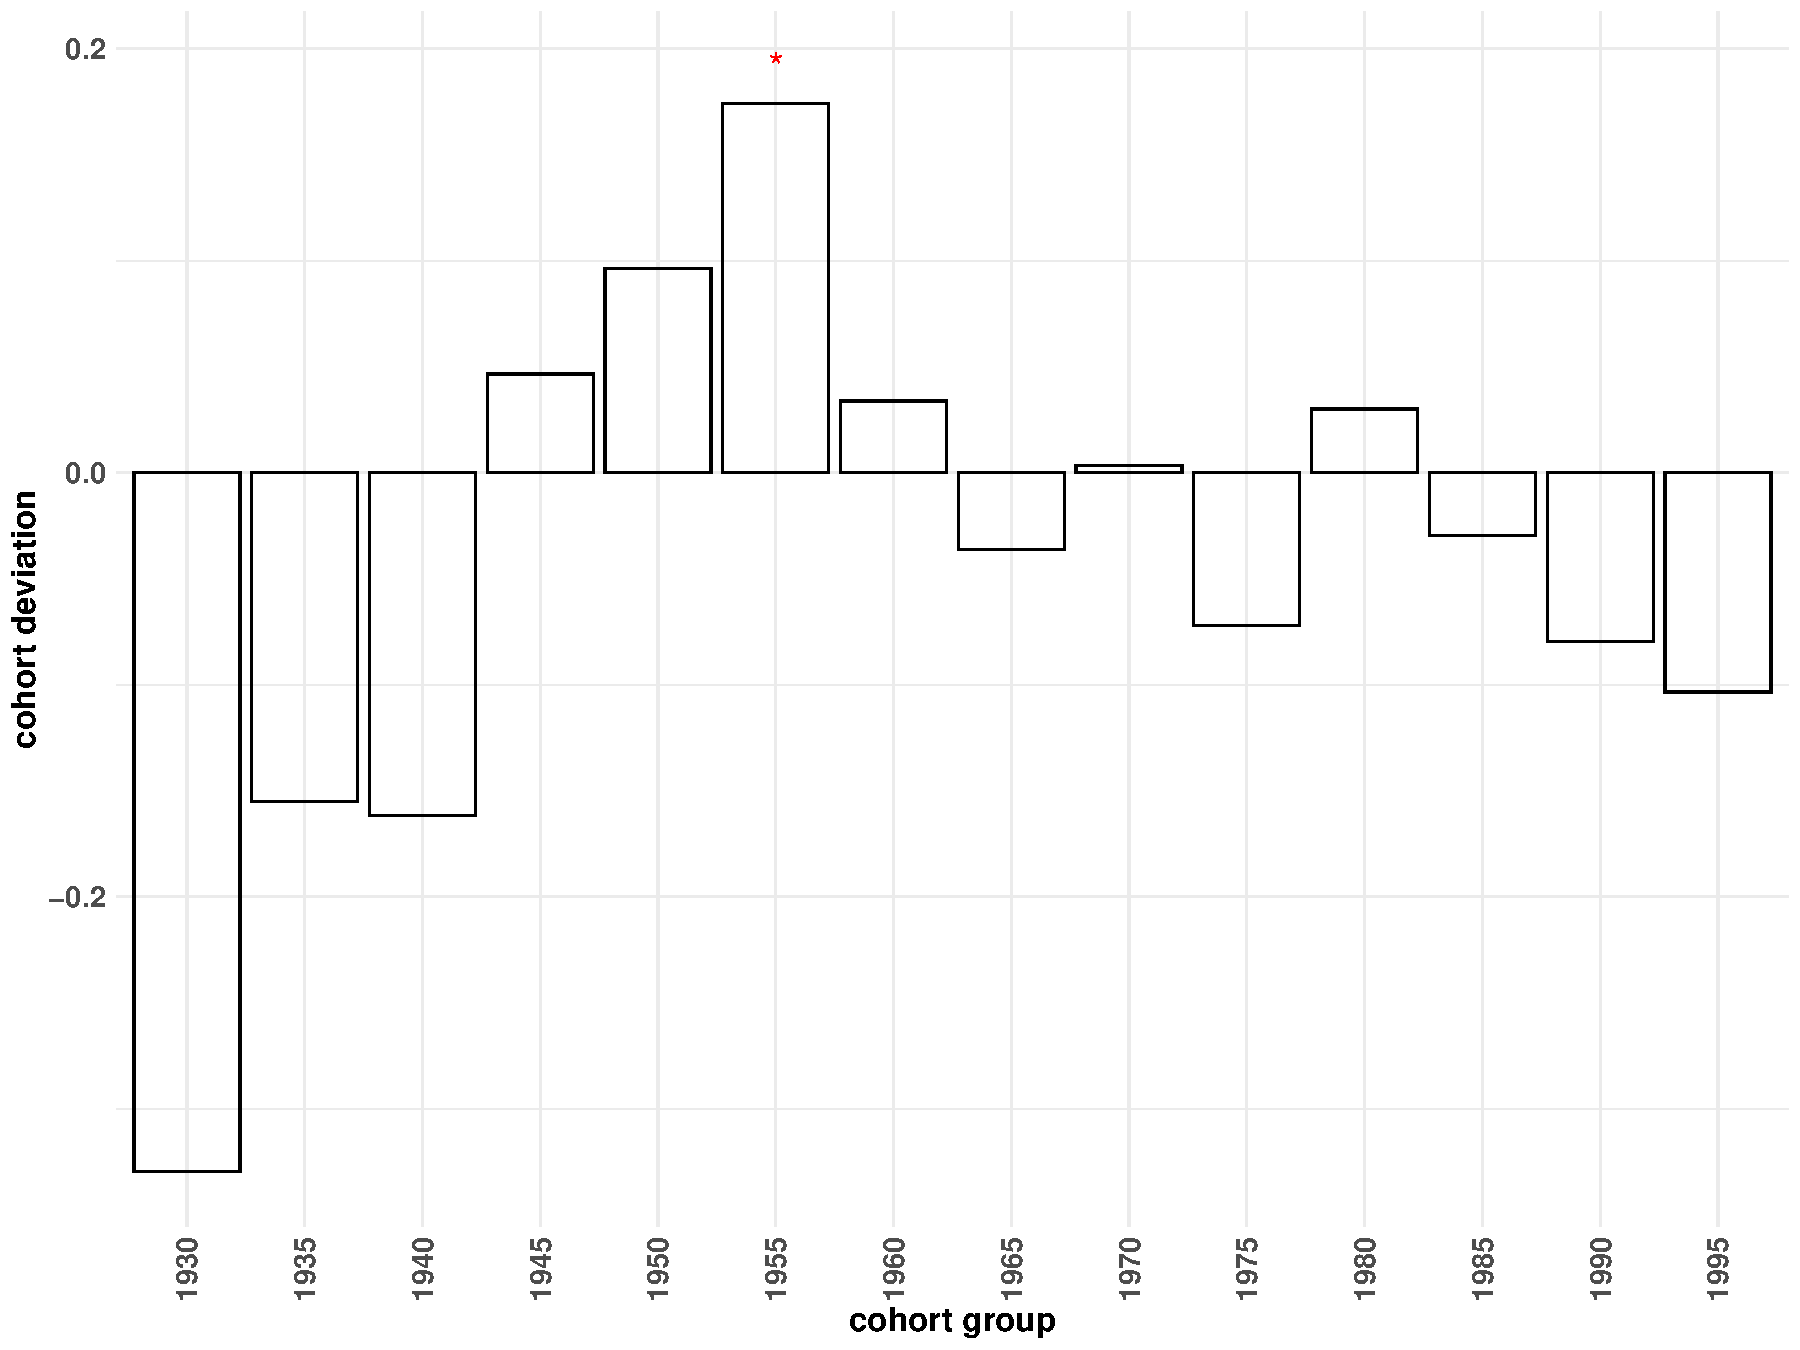
\includegraphics[width=0.8\linewidth]{figure3.pdf}
  \caption{Bar plots showing inter-cohort average deviations in women's labor force participation rates. Only the 1955 birth cohort had a significantly higher-than-expected participation rate. The horizontal line at y=0 indicates expected labor force participation rates for each cohort based on the main effects of age and period when they were observed. The bars indicate the estimated average deviation for each cohort from the age and period main effects. Bars above the horizontal line indicate positive average deviations, and bars below the line indicate negative average deviations. The asterisk sign indicates that a cohort's average deviation is significantly different from the expectation determined by age and period main effects at the .05 or lower level.}
  \label{figure:3}
\end{figure}

\hyperref[figure:3]{Figure 3} illustrates inter-cohort deviations based on the average of the age-by-period interaction estimates contained in each cohort. The horizontal line at y=0 indicates expectations for all cohort based on the main effects of age and period when they are observed. The bars indicate the estimated average deviation for each cohort from the age and period main effects. Bars above the horizontal line indicate positive average deviations, and bars below the line indicate negative average deviations. The asterisk sign indicates that a cohort's average deviation is significantly different from the expectation determined by age and period main effects. Figure 3 suggests some cohort variation in women's LFP using the 1990-2019 CPS data, but only the 1955 birth cohort had significantly higher-than-expected LFP rates. 


\subsubsection{Longitudinal data} \label{example2:gee}

For longitudinal data (i.e., panel data, repeated measure data) that include multiple cohorts, users may set the argument {\code{gee}} to {\code{TRUE}} to estimate an APC-I model using the generalized estimating equation (GEE) technique \citep{liang1986longitudinal,geerpackage}. When {\code{gee}} is {\code{TRUE}}, users will also need to specify arguments {\code{id}} and {\code{corstr}} accordingly. 

\begin{example}
> model_gee <- apci(outcome = "y",
+                  age = "age",
+                  period = "period",
+                  cohort = NULL,
+                  weight = NULL,
+                  covariate = NULL,
+                  data=simulation_gee,
+                  family ="gaussian",
+                  dev.test = FALSE,
+                  print = TRUE,
+                  gee = TRUE,
+                  id = "id",
+                  corstr = "exchangeable")
> summary(model_gee)
\end{example}

The list of output results is similar to that for pooled cross-sectional data, but the standard errors are corrected using the GEE's {\code{sandwich}} estimator. 

\section{Use the R package APCI in Stata} \label{stata}

We also designed a Stata command \code{apci} based on the Stata command \code{rcall} \citep{haghish_seamless_2019} to help implement APC-I models in Stata. The command is used as:

\code{apci} \textit{depvar} [\textit{indepvars}], outcome(\textit{depvar}) age(\textit{age}) period(\textit{period}) family(\textit{"gaussian"}) [if] [in] [\textit{weight}]


Stata users can use the above command to fit APC-I models and obtain all the results as in R. A Stata ado file for installing this command can be downloaded at \url{https://sites.psu.edu/liyingluo/software/}.


\section{Conclusion and future development} \label{conclusion}

In this article, we introduced an R package \CRANpkg{APCI} and Stata command \code{apci} for implementing the age-period-cohort-interaction (APC-I) model developed by \citet{luo_age-period-cohort-interaction_2020}. In addition to pooled cross-sectional data analysis, we extended the package to permit multi-cohort longitudinal or panel data analysis. This package also contains a set of visualization tools to help researchers motivate an APC analysis and interpret the results. We clarify the implications of coding schemes for estimating and testing main effects and interaction effects in the APC-I model. We illustrate how to use this package using the empirical examples of labor force participation using the 1990-2019 data from the Current Population Survey. 

\citet{luo_age-period-cohort-interaction_2020} described a local F test for testing the variation associated with the multiple age-by-period interactions contained in each cohort. Because the parameterization of the local F test is more intricate than it appears, the R package \CRANpkg{APCI} and the Stata command \code{apci} currently do not support such tests as of version 1.0.5 but may be available in later versions. 


Moreover, it may be of interest to examine the interaction effects of cohort and other explanatory variables such as education and geographic areas.  Because cohort effects are conceptualized and operationalized as a two-way interaction term of age and period effects, an interaction term between cohort and another variable is equivalent to a three-way interaction among age, period, and another variable. Future development may consider creating functions to facilitate summarizing and interpreting the more complex three-way interaction terms in the APC-I model.


\bibliography{APCI_manuscript_Xu_Luo}

\address{Jiahui Xu\\
  The Pennsylvania State University\\
  917 Oswald Tower
  University Park, PA 16802\\
  United States\\
  ORCiD: 0000-0003-2728-0674 \\
  \email{jpx5053@psu.edu}}

\address{Liying Luo\\
  The Pennsylvania State University\\
  202 Oswald Tower
  University Park, PA 16802\\
  United States\\
  (ORCiD: 0000-0001-5393-6695) \\
  \email{liyingluo@psu.edu}}
